%%%%%%%%%%%%%%%%%%%%%%%%%%%%%%%%%%%%%%%%%%%%%%%%%%%%%%%%%%%%%%%%%%%%%%%%%%%%%%%%
%2345678901234567890123456789012345678901234567890123456789012345678901234567890
%        1         2         3         4         5         6         7         8

\documentclass[letterpaper, 10 pt, conference]{ieeeconf}  % Comment this line out if you need a4paper
\usepackage{graphicx}
\usepackage{subcaption}
\usepackage{cite}
\usepackage{multicol}
\usepackage{url}
\usepackage{textcomp}
\usepackage{textgreek}
\usepackage{fixltx2e}


%\documentclass[a4paper, 10pt, conference]{ieeeconf}      % Use this line for a4 paper

\IEEEoverridecommandlockouts                              % This command is only needed if 
                                                          % you want to use the \thanks command

\overrideIEEEmargins                                      % Needed to meet printer requirements.

% See the \addtolength command later in the file to balance the column lengths
% on the last page of the document

% The following packages can be found on http:\\www.ctan.org
%\usepackage{graphics} % for pdf, bitmapped graphics files
%\usepackage{epsfig} % for postscript graphics files
%\usepackage{mathptmx} % assumes new font selection scheme installed
%\usepackage{times} % assumes new font selection scheme installed
%\usepackage{amsmath} % assumes amsmath package installed
%\usepackage{amssymb}  % assumes amsmath package installed

\title{\LARGE \bf
Cycloidal Geartrain In-Use Efficiency Study
}

\author{Logan C. Farrell$^{1}$, James Holley$^{2}$, William Bluethmann$^{3}$, and Marcia K. O'Malley$^{4}$% <-this % stops a space
\thanks{$^{1}$Logan Farrell is with the Department of Mechanical Engineering at Rice University and NASA: Johnson Space Center.
		{\tt\small Logan.C.Farrell@NASA.gov}}%
\thanks{$^{2}$James Holley is with the Department of Mechanical Engineering at Rice University and NASA: Johnson Space Center.}%
\thanks{$^{3}$William Bluethmann is the project manager for rovers at NASA: Johnson Space Center.}%
\thanks{$^{4}$Marcia O'Malley is on the Faculty in the Department of Mechanical Engineering at Rice University, Houston, TX}%
}


\begin{document}

\maketitle
\thispagestyle{empty}
\pagestyle{empty}

\begin{abstract}
% 7 Questions 
% 1. Focus/Problem to be Solved 
% 2. Importance - why is this important to people?
% 3. Methods - how did we test this? 
% 4. Context - talk about them in context with relevant literature and such - why do people care? 
% 5. Results - what did we show 
% 6. Unique Contribution - what is unique and why do people care? 
% 7. Possible Applications 

% 1. 
% The problem to be solved is two-fold. First, how well do single-stage cycloids of this compact pin in housing design actually work? Very little literature exists on it. The second problem is how well do two-stage cycloids work? Are they a good use of a high reduction in a small package? 
% 2.
% This is important because it adds another high reduction capability if you relax some requirements, you can get a 2x increase in specific torque with a single stage, and a huge ratio and torque capacity in a small package with a two stage if they were to actually work well. 
% 3.
% We built two test articles, a single stage, and a two-stage based on the relevant literature. We tested the single-stage for 300+ hours and 129k revolutions to determine true efficiency, run-in, and give an indication to lifetime. We ran the two-stage briefly that indicated gaps in understanding of the losses of the system, since kinematic analysis and brief force analysis are the only things laid out. So a new set of equations were developed to show loss trends in these cycloids and identify the reason of the poor efficiency of the as-built two-stage. 
% 4. 
% 
% 5. Results 
% The compact single stage cycloid showed efficiencies similar, and slight above those published by Harmonic drive. In addition, a notable burn in time was required before steady state performance was reached and through the 300 hours of running, no appreciable loss of efficiency was seen. Also, the efficiency was not flat with torque.  For the two-stage cycloids, the loss calculations show that, to achieve any reasonable efficiency, the lobe to pin interactions should be made from rolling elements, and the theoretical calculations fall in the same region as the actual system performed, substantiating those claims. 

% 6. Unique Contribution 
% To this point, very little testing has been done on a single-stage cycloid, only about 80 minutes. This long duration testing shows that high efficiencies (80%), similar to harmonic can be achieved for substantial amounts of time. This validates this drive as a possible replacement for harmonic in cases where backlash is acceptable. Additionally, very little aside from basic kinematic analysis of the two-stage concept has been performed. This analysis gives design recommendations that were not previously published, allowing designers to design better two-stages. 

% 7. Possible Applications 
% This shows that single-stage cycloids of the compact style could be used to replace harmonic drives in cases where backlash is acceptable. Additionally, the high reuduction drives, if made with rolling elements, could potentially have pretty high efficiencies and could provide a very nice high reduction compact package. 
\begin{center}
\large
\textbf{Abstract}
\end{center}

Many robotic applications demand compact, high reduction drives for their actuators. To date, the most commonly used actuator for this application is a harmonic drive. However, cycloidal drives could be considered for these applications as they provide high reductions in a compact package, are highly customizable, and can be easily manufactured in comparison to harmonic drives. Single-stage cycloids have been well analyzed in the literature, but not well tested. In this work, a single-stage cycloid was built and run for 300+ hours and 129,000 output revolutions to determine in-use efficiency and lifetime. This testing demonstrated that the compact, pin-in-housing designs can achieve efficiencies near and above the efficiencies of a comparable harmonic drive with a peak efficiency of 81\% as well as a 2x increase in specific torque. A substantial burn-in of approximately 8 hours was noted, and the efficiency did not degrade appreciably over the course of the testing. A new design for a two-stage cycloid has been recently proposed and the basic kinematic analysis conducted. A test article for this two-stage design was constructed and tested. This testing identified gaps in the literature regarding the losses associated with the lobe to pin interactions. This work developed the mathematics necessary to characterize these losses in theory and are then compared to the tested actuator. The actuator's losses nearly match the predicted losses of the two-stage system. This work presents many additional design equations for a two-stage cycloid system, the primary result suggesting that a two-stage system must be built with rolling elements in the housing to achieve satisfactory (above 50\%) efficiencies. This thesis demonstrates enables two key conclusions: first single-stage cycloids are a viable replacement for harmonic drives in high reduction applications where backlash is allowed, second, additional design equations are necessary for a two-stage cycloid design.
\end{abstract}

\section{Introduction}
\label{intro}
A robot operating in an unstructured environment is faced with a plethora of challenges, each at the frontier of what is possible with modern robotics.
Recently, much work has gone into understanding how to command and control a robotic system inside the wide range of novel, complex environments that occur in domains such as disaster relief~(e.g., \cite{Johnson2015}), caregiving~(e.g., \cite{FISCHINGER201660}), and spacecraft logistics~(e.g., \cite{Baker2017}).
These systems must integrate many disparate components of robotics technology and reliably use them: object detection and localization, task and motion planning, and human-robot interfaces.
Each of these systems employs their own methods of composing these parts into a usable whole.
Additionally, human operators must be able to command these robots to achieve real work.
How to integrate these components together for a complex system with many degrees of freedom in a unstructured environment is an open question.

\begin{figure}
  \centering
  \includegraphics[width=0.5\textwidth]{fig/Figure_01/Figure_01.jpg}
  \caption[Robonaut 2 Executing Various Tasks] {
    \label{fig:r2_tasks}
    Robonaut 2, a dexterous humanoid robot developed by NASA / GM, executing tasks with the proposed system.
  }
\end{figure}

\begin{figure*}
  \centering
  \begin{subfigure}[t]{0.35\textwidth}
    \includegraphics[width=\textwidth]{fig/Figure_02/Figure_02.jpg}
    \caption[Robonaut 2 in Mock-Up Space Station]{
      \label{fig:scenario_real}
    }
  \end{subfigure}%
  \begin{subfigure}[t]{0.6\textwidth}
    \includegraphics[width=\textwidth]{fig/Figure_02/Figure_02.png}
    \caption[Breakdown of Task at Hand]{
      \label{fig:scenario_drawing}
    }
  \end{subfigure}
  \caption[Archetypal Scenario for the System] {
    \label{fig:scenario}
    An example task that the system should solve.
    \textbf{a)} Robonaut 2 in a microgravity simulator at NASA Johnson Space Center~\cite{Valle2011}.
    \textbf{b)}
    i) R2 starts at one end of the mock-up station,
    ii) climbs towards the valve,
    iii) positions torso by hatch while grasped with both feet,
    iv) and turns the valve and pushes the hatch away.
    v) R2 then climbs through the hatch,
    vi) positions torso in by the rack while grasped with both feet,
    vii) unbuckles the restraint,
    viii) and removes the bag from the rack.
  }
\end{figure*}

Technologies presented in the literature are generally demonstrated in isolation, not part of a systemic whole.
Recently, studies and reports of integrating these technologies shows the additional challenges to consider when designing a system of this nature, such as how to handle the failure of any individual component within the context of the greater whole.
For example, it is a challenge to transform under-specified user input into usable queries by an autonomous planning layer.
This must be addressed in order to have usable high-level actions.
Another challenge is to communicate inferences the system has made about its environment to a user (e.g., recognized objects and ways to manipulate them).

This work has been demonstrated on is the Robonaut 2 (R2) system~\cite{Diftler2011}, depicted accomplishing tasks in Figure~\ref{fig:r2_tasks}.
Resources are limited in spacecraft, creating need for a system can reuse human tools and spaces.
R2 is a robotic platform designed to work in the same space as humans in spacecraft.
Future NASA mission concepts also require spacecraft to be uncrewed for extended periods of time, but systems inside still require maintenance.
R2 has two arms with seven degrees of freedom (DoF) and a 12 DoF hand each, a three DoF neck, a waist joint, and two seven DoF legs with end-effectors designed to interface with spacecraft handrails.
R2 also has a sensor package within its head and at the end of each leg that gives image and depth data.
Despite its humanoid form, R2 is more akin to a mobile manipulator with multiple end-effectors, providing an excellent testbed for the technologies needed to command complex tasks in unstructured environments. 

This paper presents a software system capable of solving motion planning problems with a variety constraints through a single set of interfaces, enabling high- and low-level task specification.
The system design problem and an archetypal problem the system should solve is shown in Section~\ref{sec:problem}.
The presented system is shown in Section~\ref{sec:system}, and a case study presenting the system solving the archetypal problem is shown in Section~\ref{sec:study}.
Finally, a summary of lessons learned is given in Section~\ref{sec:lessons}, with concluding remarks in Section~\ref{sec:conclusion}.


\section{Cycloid Design}
\label{design}
\begin{table*}[t]
  \vskip0.2cm
  \caption{Designed Duty Cycles for System}
  \label{duty_cycle}
  \begin{center}
    \vskip-0.2cm
    \begin{tabular}{|c||c||c| |c| |c|}
    \hline
    Time Used & Output Torque (Nm) & Output Speed (RPM) & Actuator Torque (Nm) & Actuator Speed (RPM)\\
    \hline
    5\% & 2440 & 6.8 & 554.7 & 33.9\\
    \hline
    20\% & 1627 & 6.8 & 369.8 & 33.9\\
    \hline
    60\% & 542 & 15.3 & 123.3 & 76.3\\
    \hline
    15\% & 135 & 15.3 & 30.8 & 76.3\\
    \hline
    \end{tabular}
  \end{center}
\end{table*}

In 2007 and 2008, NASA developed a manned rover prototype for planetary surfaces for future missions \cite{ref:rover}.
This robotic vehicle is made up of six independent wheel modules, each with their own drive, steering, and both active and passive suspension.
In 2014, a new prototype wheel module was designed and created to analyze potential technologies that could be used in these applications.
In the new design layout, it was possible for the drive wheels to counter-rotate against the steering and put large shock loads into the steering system.
These requirements called for a compact package, high load, high shock load, and tolerance of backlash lent themselves to the selection of a cycloidal drive for the steering actuator.
The prototype wheel module layout can be seen in Fig \ref{wheel_module}.

\begin{figure}[t]
   \centering
   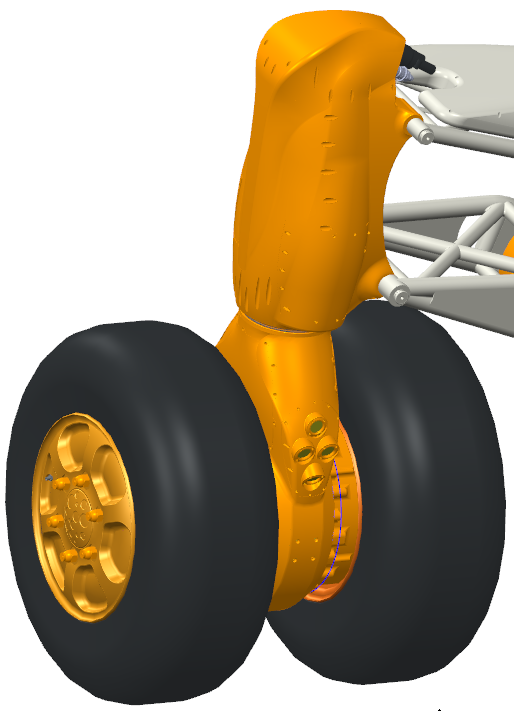
\includegraphics[width=0.40\linewidth]{fig/wheel_module_CAD}
   \caption{CAD model of rover wheel module prototype.
   Suspension arms hold the steering column.
   Each wheel has an in-wheel drive motor.}
   \label{wheel_module}
\end{figure}

Based on the load cases, the actuator was required to output a stall torque of 2,440 Nm (1800 ft-lb) with a max output speed of 1.57 rad/s (90 deg/s) at 1,626 Nm (1200 ft-lb).
The required torque/speed data points are presented in Table \ref{duty_cycle} with an assumed loss of 88\% chosen based on the available literature.
The actuator layout for the vehicle placed the motor and cycloid off center of the steering axis with an additional 5:1 reduction into the steering column, thus decreasing the torque needed for the cycloid output, but increasing the potential shock loading.

Many sources have laid out the design parameters for these drives and the equations are provided below for completeness.
Shin and Kwon \cite{ref:on_the_lobe} presented the mathematical definition of the cycloid profile as

\begin{equation} \label{eq:0}
Z = \frac{Z_1} {Z_2 - Z_1}
\end{equation}
\begin{equation} \label{eq:1}
C_x = R cos\phi -R_r cos(\phi + \psi) - e cos((Z_1 + 1)\phi) 
\end{equation}
\begin{equation} \label{eq:2}
C_y = -R sin\phi + R_r sin(\phi + \psi) + e sin((Z_1 + 1)\phi) 
\end{equation}
\begin{equation} \label{eq:3}
\psi = tan^{-1} \lbrack\frac{sin(Z \phi)}{cos(Z \phi) - R / (e(Z + 1))}\rbrack 
\end{equation}

where \textit{Z} is the overall reduction, \textit{Z\textsubscript{1}} is the number of lobes, \textit{Z\textsubscript{2}} is the number of pins, \textit{R} is the distance from the center to the rollers, \textit{R\textsubscript{r}} is the diameter of the pins, \textphi\ is the angle of the input shaft and \textpsi\ is the angle of contact between the outer pin and the cycloid lobe.

Using both the formula for the reduction in diameter of the cycloid disk to account for machine tolerances \cite{ref:machine_design} \cite{ref:design_and_application} as well as Ye et al.'s formula for calculating the limit of undercutting \cite{ref:ye}, the allowable sizes of the profiles and pins can be determined.
Sensinger \cite{ref:unified_approach} laid out simple equations for calculating stress on the lobes and pins that has been further modelled and studied by others.
The force on the cam for calculating the bearing load with eccentricity e, ratio Z , and torque T is

\begin{equation} \label{eq:4}
F_{cam} = \frac{T}{e Z}.
\end{equation}

The simplified stress equations where \textit{t} is the contact thickness, and \textit{b} is the width of contact determined by (\ref{eq:7}) and (\ref{eq:8}) are

\begin{equation} \label{eq:5}
F = \frac{T}{R - R_r}
\end{equation}
\begin{equation} \label{eq:6}
\sigma = \frac{2F}{\pi b t} (3 + 4v^2)
\end{equation}
\begin{equation} \label{eq:7}
b = \sqrt{\frac{4F (v-v_1^2) /E_1 + (1 - v_2^2)/E_2}{\pi l (1/R_1 + 1/R_2)}}
\end{equation}
\begin{equation} \label{eq:8}
R_2 = \frac{(R-eZ - e)^3}{R-e(Z-1)^2} - R_r.
\end{equation}

\begin{figure}[!b]
   \centering
   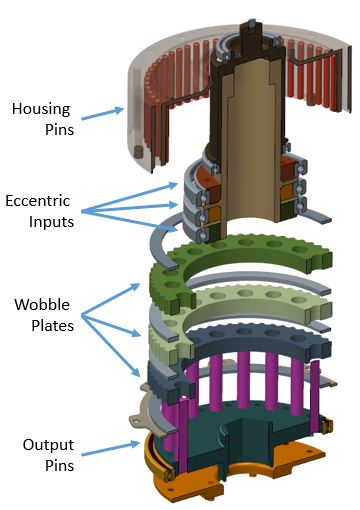
\includegraphics[width=0.7\linewidth]{fig/exploded_labeled}
   \caption{Exploded view of the cycloidal reducer.
   Three wobble plates are driven by the input shaft with 120\textdegree\ offsets.
   The ring pins are are free pins inserted in the housing.
   The output has pins run through all three wobble plates to harness the counter-rotation for the drive output.}
   \label{cycloid_exploded}
\end{figure}

The stress calculations and trading of overall size and ratio led to a necessary plate thickness of 2.38cm (0.9375in).
Instead of a single large plate, three wobble plates were selected to split the load on the central input shaft across three bearings as well as to build in natural balance for the actuator.
If a single plate is used, a counterbalance must be added to avoid substantial vibration.
In this case, the three plates were offset 120\textdegree\ to balance these loads and vibration.
This adds stack height to the system to allow separation between the plates.
This arrangement allows the large design loads to be able to be handled by the system.
The exploded view of this design can be seen in Fig \ref{cycloid_exploded}.

The actuator uses a Parker Frameless Kit Motor, model K089200-7Y with no hall effect sensors and is commutated using a Renishaw RM-44 magnetic incremental and absolute position sensor.
The final reduction is 59:1 followed by the final 5:1 output gear.
The system is commutated using the delta hysteresis commutation scheme and PI velocity control was implemented to maintain constant motor speeds \cite{ref:electric_machines}.



\section{Experimental Methods}
\label{methods}
\begin{figure}[!b]
   \centering
   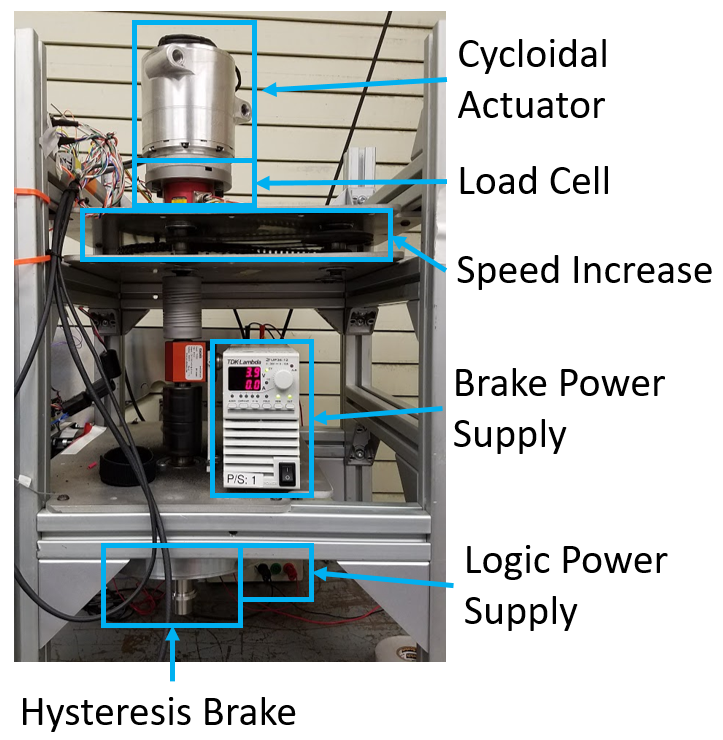
\includegraphics[width=0.75\linewidth]{fig/test_stand}
   \caption{Experimental Test Setup.
   The cycloid actuator is mounted to structure via the load cell.
   There is a speed increase so the brake can generate enough torque on the system.
   Not pictured is the controlling computer, motor driver, and high voltage supply.}
   \label{test_setup}
\end{figure}

The intent of testing the cycloidal drive is to experimentally determine and compare the in-use efficiency results to the published performance data for a comparable harmonic drive.
To accomplish this, the actuator was mounted to a Futek TF600 5000inlb load cell to measure output torque of the actuator.
The load cell signal was collected through a analog to digital converter and converted to standard units on the motor driver.
A verification of torque readings was completed using a calibrated torque wrench to ensure accuracy of the conversion.
Load was regulated by a Magtrol HB-1750 hysteresis brake.
A 36:1 speed increase was added via three chain stages between the output of the actuator and the hysteresis brake to achieve the desired applied loads.
The hysteresis brake was powered using a separate 24V Lambda-TDK power supply that was controlled through a RS-485 communication link to the test computer.
NASA's 'turbodriver' motor driver was used for commanding motor currents.
The motor driver was powered by a TDK-Lambda 12V supply for logic power and a TDK-Lambda 150V and 5A supply for high voltage power.
A hysteresis current controller was used on the motor drive to accurately provide torque producing current to the motor.
The motor driver monitored the actuator power by measuring torque from the load cell and speed with an incremental encoder located at the actuator motor shaft.
The test computer monitored the high voltage supply and recorded voltage and current to determine input power to the system and recieved data from the motor driver to calculate output power.
The test setup is shown in Fig \ref{test_setup}.

Due to the tightly integrated actuator design, the motor and cycloid cannot be separated to purely isolate the losses in the cycloid.
The efficiency map of the motor over its torque and speed range was provided by Parker Motors.
For calculation purposes, this table is used as a lookup table for efficiency of the motor given the current motor velocity and rms input current.
While this does generate a level of uncertainty in the data, these motors are mass manufactured and defects are assumed to be small.
The error in the motor efficiency map is assumed to be small and would not influence the perceived trends and results.
Power losses in the motor driver were also taken into consideration by calculating power losses in the IGBT that drives the motor.
Instantaneous current draw and a switching frequency of 12 kHz were used for the calculation, neglecting small leakage losses \cite{ref:IGBTPower}.

\begin{figure}[!b]
   \centering
   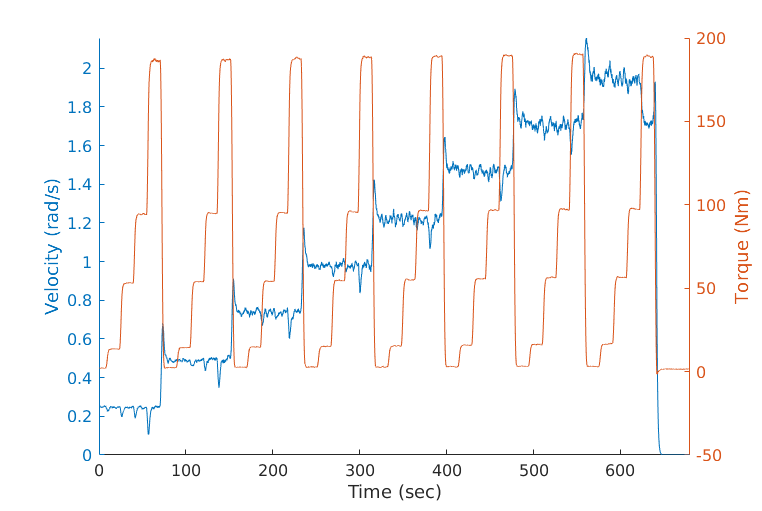
\includegraphics[width=\linewidth]{fig/eff_test_profile_v4}
   \caption{Testing profile for efficiency.
   At each speed step, torque is ramped up through five different levels, then the speed is increased.
   At the last step, the maximum of the supply was reached so motor velocity dropped.}
   \label{eff_profile}
\end{figure}

The system was tested in two separate ways, an efficiency cycle and a long term drive cycle.
The efficiency cycle test was run after the long term drive cycle to ensure steady state performance before cycling through a set of velocities and torques.
The actuator is subjected to eight velocity steps increasing 0.25 rad/s each time.
In each velocity step, the torque is ramped up and maintained for 15 seconds at values of 1Nm, 15Nm, 52Nm, 94Nm, and 189Nm.
This testing profile can be seen in Fig \ref{eff_profile}.
The long term drive cycle was run continuously each day for 6 to 12 hours with the duty cycles shown in Table \ref{table_2}.
The total runtime of the system, not including the initial checkout and verification of the actuator, has been 111 hours.

\begin{table}[h]
  \vskip0.2cm
  \caption{Long Run Drive Cycle}
  \label{table_2}
  \begin{center}
    \vskip-0.2cm
    \begin{tabular}{|c||c||c|}
    \hline
    Time (s) & Velocity (rad/s) & Torque (Nm)\\
    \hline
    150 & 1.0 & 0.0\\
    \hline
    150 & -1.0 & 0.0\\
    \hline
    60 & 0.5 & 26.0\\
    \hline
    60 & -0.5 & 26.0\\
    \hline
    150 & 1.5 & 10.0\\
    \hline
    150 & -1.5 & 10.0\\
    \hline
    30 & 1.0 & 50.0\\
    \hline
    30 & -1.0 & 50.0\\
    \hline
    300 & 0.5 & 18.0\\
    \hline
    300 & -0.5 & 18.0\\
    \hline
    \end{tabular}
  \end{center}
\end{table}

It should be noted that the actuator was used briefly in the robot validation after initial development and construction of the prototype wheel module.
The total time of use was approximately three hours.
Afterwards, it was removed from the wheel module and subjected to the characterization that is discussed in this work.
The motor has a continuous current rating of 4.3 A\textsubscript{rms} and a peak rating of 15A\textsubscript{rms}.
The actuator was designed to be liquid cooled to allow operations above the continuous values, but this could not be achieved during testing.
For long duration testing, the torque values were decreased to avoid thermal issues.
The motor was tested to approximately 6A\textsubscript{rms} during efficiency testing due to the limit of the power supply.
Also, the motor driver's rated limits are 150V, therefore the actuator's maximum rated speeds could not be tested.
The nominal cycle of the actuator as seen in Fig \ref{duty_cycle} is still achievable and has been tested.

\begin{figure*}[t]
   \centering
   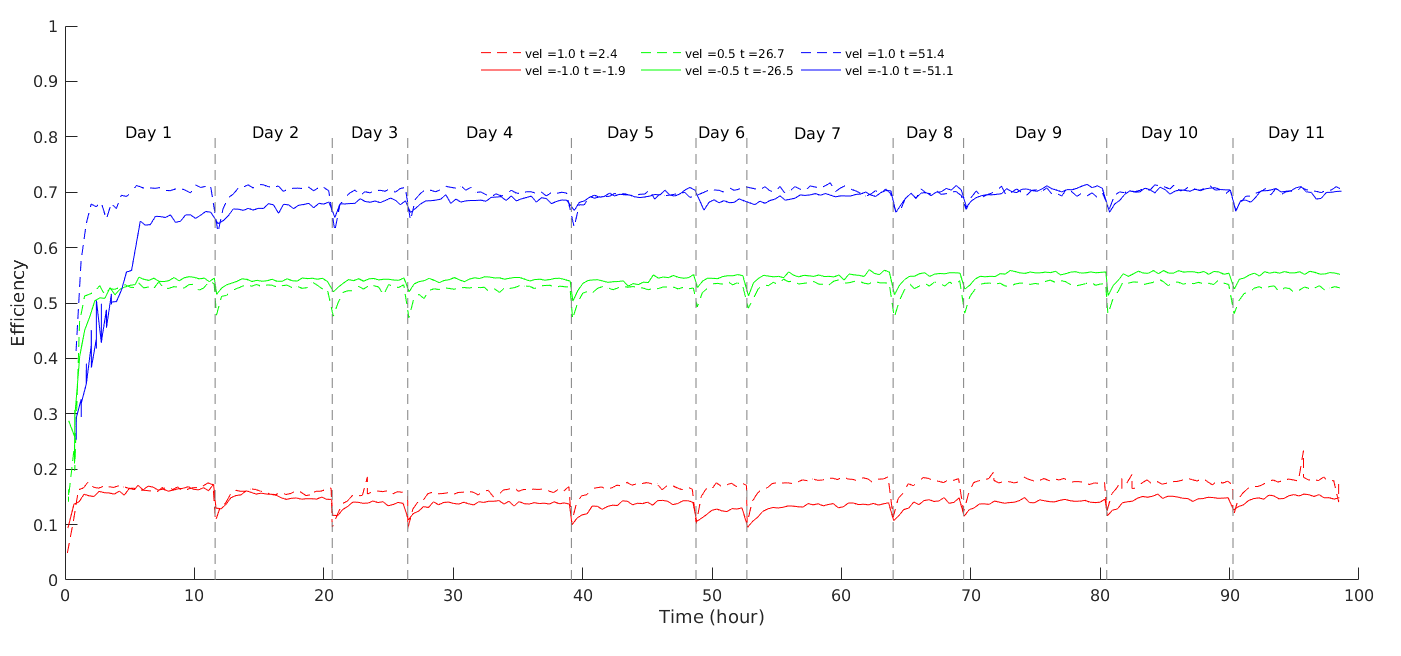
\includegraphics[width=\linewidth]{fig/long_run_plot_v4}
   \caption{Efficiency over time for three different speed/torque profiles during the drive cycle.
   The forward motion can be seen with the dotted line, reverse with the solid line.
   At the onset of testing, visible efficiency gains are made.
   As each day begins, there is a clear warm-up period before steady state.
   }
   \label{long_run}
\end{figure*}



\section{Results}
\label{results}

\begin{figure*}[t]
   \centering
   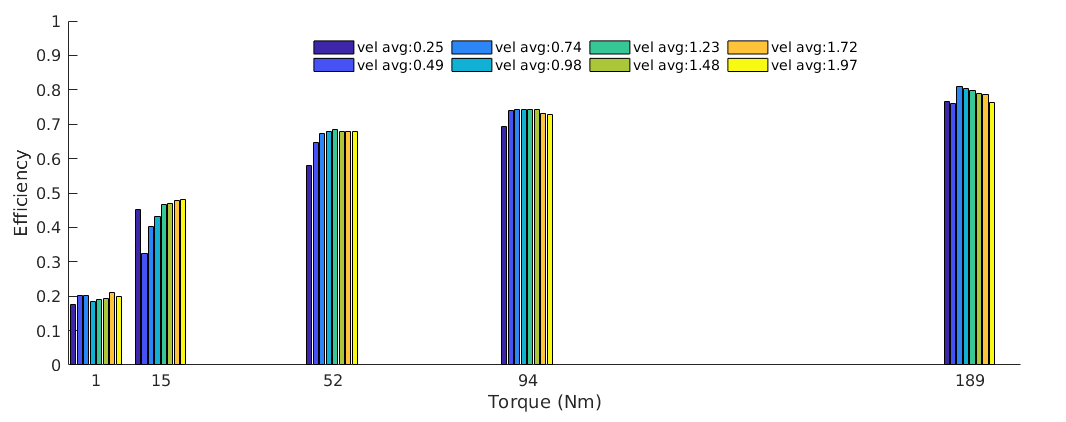
\includegraphics[width=0.8\linewidth]{fig/eff_test_bar_plot_v3}
   \caption{Grouping of average efficiencies at each torque step.
   Efficiency depends heavily on torque, and slightly on speed.}
   \label{eff_results}
\end{figure*}

Duty cycle testing was performed first on the actuator.
These tests were done at lower torques to prevent the motor from overheating to allow extended duration testing.
The total test time prior to these duty cycle tests was approximately 5.2 hours to bring up and check out the actuator testbed system.
Once this checkout was complete, the 100 hours of duty cycle testing were conducted over the course of 11 days with the drive cycle presented in Table \ref{table_2}.
Three of the torque/speed combinations in forward and reverse are plotted on Fig \ref{long_run} to show the general characteristic trends seen in actuator performance.

After this duty cycle testing to ensure the actuator had sufficiently broken-in and achieved steady state performance, as evident by Fig \ref{long_run}, the pure efficiency cycles were run.
A profile of speeds and torques (see Fig \ref{eff_profile} were run on the actuator to show the relationship between speed, torque, and efficiency.
This profile was run three times and the results at each torque and speed combination were averaged (see Fig \ref{eff_results}.


\section{Discussion}
\label{discussion}
The efficiency of the system is dependant on the torque through the gearbox as shown in Fig \ref{eff_results}.
This contradicts previous studies that suggested that cycloidal drives have a constant efficiency across the torque range.
There is also a much less pronounced relationship between the velocity and the cycloid efficiency that can be noted in the torque bands.
This result suggests that the cycloid efficiency behaves more like a planetary or harmonic drive gearbox in its efficiency profile.
A comparison of cycloid, harmonic, and planetary efficiency profiles can be seen in Fig \ref{eff_comp}.
The figure shows the efficiency for a harmonic drive CSF-45-50-2UH-LW \cite{ref:harmonic_sheet} which has a comparable ratio and torque capability to the tested cycloid and weighs 5.1kg, and a representative planetary efficiency curve from the engineers at Maxon Motor.
If backlash is acceptable in a system, a cycloidal drive can provide similar or better efficiency profiles to a harmonic drive while providing a potential 2x increase in specific torque (Nm/kg).

\begin{figure}[t]
   \centering
   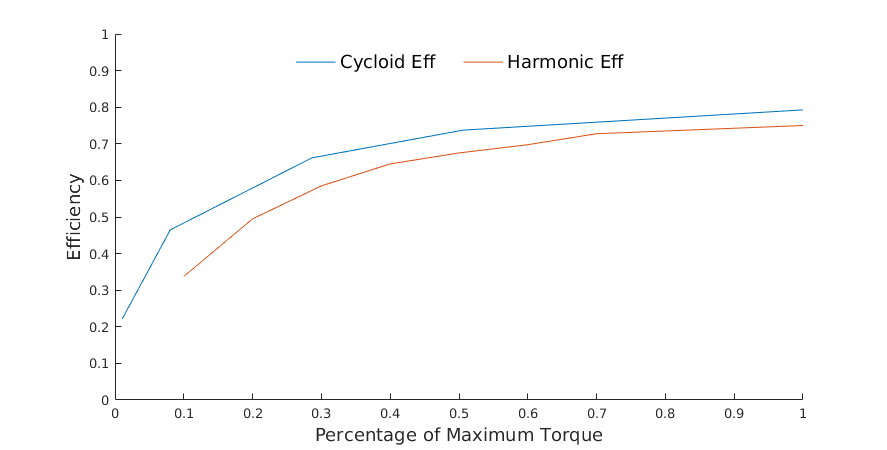
\includegraphics[width=\linewidth]{fig/eff_comp_v3}
   \caption{Comparison of efficiency over maximum torque rating of the tested cycloid, a comparable harmonic drive, and a theoretical planetary gearset.
   The cycloid exhibits the same efficiency increase over torque range and has a comparable and slightly higher efficiency than the harmonic.}
   \label{eff_comp}
\end{figure}

There was a substantial break-in time for the actuator before steady state results were achieved (see Fig \ref{long_run}).
In the high torque case, specifically in the reverse direction, there was an approximately linear increase in efficiency over the course of the first seven hours of duty cycle testing.
This testing began after a minimum of five hours of run time spread out through many short sessions while getting the test system running.
The large increase in efficiency can be noted in the other lower torque profiles as well, starting well below their final steady state values.
The authors theorize that this is due to break-in of the manufactured parts required because of machining inaccuracies.
Due to the complex interaction required of the trochoidal motion profile, slight manufacturing deficiencies could cause build-ups of stress and loss in particular points on the drive.
It would make sense that these could manifest in one direction and not the other if a lobe was misshapen on the trailing edge in one direction, it would be the lead in the other, causing the additional loss.
Through the first hours of testing, these materials likely wore in to each other until the contact was smooth, resulting in the more readily achieved steady state efficiencies in subsequent hours of testing.

Additionally, there is a marked improvement over the first 30 minutes of runtime in the efficiency of the system.
This is likely due to the grease and heat in the system.
The gearbox is greased with Lucas Oil Red'N'Tacky which has a viscosity index of 86 min.
This was chosen because it is designed for high loads for extended periods of time in gear and sliding surface applications, as well as ease of use for Earth testing and verification.
Therefore, during the warm-up period as the actuator temperature increases, the viscosity decrease is likely enough to cause a notable increase in efficiency of the system.
The authors leave the study of a lower viscosity grease's effect on performance, as well as grease suitable for vacuum, for future work.



\section{Conclusion}
\label{conclusion}
To enable a complex mobile manipulator to do useful work under operator guidance, a software system that ties together high-level modules, composed of other, lower-level components.
The core contribution of this paper is the development of the interaction between these modules, and the capabilities they should provide to accomplish complex tasks in an unstructured environment.
These modules were 
  \textbf{a)} the underlying robot that provides some guarantees of complaint motion,
  \textbf{b)} task and motion planning to generate feasible,
  \textbf{c)} object handling via computer vision and object-associated semantics,
  \textbf{d)} and a user interface for a user to specify both high- and low-level goals for the system.
The specific implementation presented was demonstrated within a archetypal logistics task in a mock-up space station, and shown to be efficient for many complex tasks.
These modules are largely robot-independent, with robot-specific implementation coming only into play at the task and motion planning layer, which can solve a wide variety of complex, constrained motion planning requests, streamlining the design of other modules within the system.



\section{Acknowledgements}
\label{acknowledgements}
\begin{center}
\large
\textbf{Acknowledgments}
\end{center}

First, I would like to thank my advisor, Dr. Marcia O'Malley. Thank you for taking a chance on a new student you had only met on the phone. And a huge thank you for the amazing amount of help, guidance, and time to work towards my degree. Without Dr. O'Malley, I'm confident I would not have been able to accomplish this degree. Also, I would like to thank the support I received from the entire MAHI lab at Rice. The support you all provided was pivotal through the coursework, but the very valuable friendships that have been formed were an even larger help. 

I would also like to thank all of my co-workers and managers at NASA: Johnson Space Center. To my managers, thank you for helping me set up this opportunity, and allowing me the time needed to attend courses and work on the thesis. For my co-workers, thank you for supporting me and picking up slack when I had to go to meetings, class, and other commitments on campus, I really appreciate it. And most of all, thank you to Mason Markee, Ed Herrera, and Anthony Lapp for the inspiration and foundation to begin the work on cycloids. 

And of course, I would like to thank my family. Thank you to my parents who have provided me with so many of the opportunities that allowed me to reach this point. Without your guidance and support, I wouldn't be where I am. On top of that a special thanks for reading all of this and helping find my grammatical errors!
Finally, I would like to thank my fianc\'e, Krista, for her support through this whole process, especially for letting me off the hook for a lot of the wedding planning to finish this thesis. I look forward to repaying the favor for the rest of our lives. 

\bibliographystyle{IEEEtran}
\bibliography{Cycloid_ICRA_Bib}

\end{document}
